\documentclass[UTF8,a4paper,zihao=5,fontset=fandol]{ctexart}
\usepackage[top=20mm,bottom=21mm,left=22mm,right=22mm]{geometry}
\usepackage{amsmath,amssymb,booktabs,tabularx,array,multirow,graphicx,xcolor,caption,cite,placeins,float,hyperref}
\setmainfont{TeX Gyre Termes}
\setsansfont{TeX Gyre Heros}
\hypersetup{colorlinks=false,pdfborder={0 0 0.6},linkbordercolor={1 0 0},citebordercolor={0 1 0},urlbordercolor={0 1 1},pdfhighlight=/I,bookmarksnumbered=true,pdftitle={基于域内预训练与空间条件融合的DAPI虚拟染色},pdfauthor={通信速通生物}}
\ctexset{section={format=\large\bfseries,beforeskip=11pt,afterskip=6pt},subsection={format=\normalsize\bfseries,beforeskip=8pt,afterskip=4pt},subsubsection={format=\normalsize\bfseries,beforeskip=6pt,afterskip=3pt}}
\captionsetup{font=small,labelfont=bf,labelsep=period,skip=5pt}
\setlength{\parskip}{2pt}\setlength{\parindent}{2em}
\setlength{\emergencystretch}{2em}
\setlength{\textfloatsep}{11pt plus 2pt minus 2pt}
\setlength{\dbltextfloatsep}{12pt plus 2pt minus 2pt}
\setlength{\abovedisplayskip}{6pt}\setlength{\belowdisplayskip}{5pt}
\postdisplaypenalty=10000
\raggedbottom
\renewcommand{\arraystretch}{1.13}\linespread{1.06}
\newcolumntype{Y}{>{\raggedright\arraybackslash}X}
\newcommand{\op}[1]{\operatorname{#1}}
\newcommand{\sym}[1]{\par\nobreak\noindent\begin{minipage}{\linewidth}#1\end{minipage}\par}
\newcommand{\code}[1]{\texttt{\detokenize{#1}}}
\definecolor{enc}{HTML}{D9E6DD}
\definecolor{dec}{HTML}{F2DFCA}
\definecolor{cond}{HTML}{E6E0EF}
\definecolor{light}{HTML}{F2F2F2}
\pagestyle{plain}
\begin{document}
\begin{center}
{\LARGE\bfseries 基于域内预训练与空间条件融合的 DAPI 虚拟染色}\par
\vspace{9pt}
{\large 通信速通生物}\par\vspace{5pt}
通信速通生物\quad AIC-2026-51865112\par
\vspace{9pt}
\end{center}

\begin{abstract}
针对肝脏 DAPI 图像到免疫标记图像的虚拟染色任务，本文构建融合局部上下文与空间条件的四通道预测网络。网络以 ConvNeXt V2 为主干，通过跳跃连接与像素重排恢复分辨率，并以 DAPI 统计特征和邻域缩略图调制瓶颈特征。完整流程包括按组织区域划分数据、DAPI 域内掩码重建预训练、五折教师监督训练与折外目标生成、全量学生监督训练与知识蒸馏，以及固定几何视角推理。学生先学习真实标签，再以真实标签损失和教师预测蒸馏损失的加权和训练；推理仅使用该学生模型，将两个平移视角下的旋转、翻转预测恢复至原坐标并等权平均，输出 CD45RO 图像。五折教师对照中，域内预训练带来 1.03110 的综合分数增益；最终全量学生的平台综合分数为 79.1052，SSIM 为 0.899，PSNR 为 26.932 dB。
\end{abstract}

\FloatBarrier
\section{任务背景与方法概览}\label{sec:overview}
本节介绍 DAPI 虚拟染色任务，并概述网络设计及训练、推理流程。
DAPI 图像提供细胞核及其空间分布信息，虚拟染色模型通过配对训练学习这些形态信息与目标免疫标记之间的关系。本方案面向肝脏数据，联合输出 CD68、CD45RO、HLA-DR 和 Vimentin。训练目标偏重 CD45RO，其余通道通过共享特征参与监督。

网络采用 U 型多尺度特征融合思路\cite{unet}，参考 Cytoland 中面向显微图像翻译的 UNeXt2 设计\cite{cytoland}，以 ConvNeXt V2 块构建编码器和解码器\cite{convnext}。域内预训练采用全卷积掩码自编码（fully convolutional masked autoencoder，FCMAE）目标。上采样采用子像素重排\cite{espcn}，条件注入采用特征逐通道线性调制（feature-wise linear modulation，FiLM）\cite{film}。本文在上述结构基础上构建 DAPI 统计与空间缩略图双分支，并通过基于图像回归的知识蒸馏，将教师预测作为学生的辅助监督。

这些设计分别对应三类信息需求：上下文扩展提供目标图块之外的真实相邻像素，邻域缩略图补充较大范围的组织背景，域内预训练利用训练 DAPI 的重建信号学习表征。在此基础上，知识蒸馏使用按组织区域留出的教师预测作为软目标。蒸馏发生在学生训练的第二阶段：真实标签损失与 CD45RO 教师预测损失分别占 0.8 和 0.2，教师信息由此进入最终学生的参数。

图\ref{fig:workflow}概括了从训练到部署的流程。首先按组织感兴趣区域（region of interest，ROI）划分五折，并从同一 ROI 内的 DAPI 构造上下文与空间条件；随后以公开编码器权重为起点，在各折训练 DAPI 上进行域内预训练，再用配对标记图像训练教师。每个教师仅预测其留出 ROI，五折预测汇集为覆盖全部训练图块的教师目标。最终学生另用全量训练 DAPI 进行域内预训练，先以真实标签完成第一阶段监督训练，再在第二阶段加入教师目标。部署时固定学生参数，对测试 DAPI 进行多视角预测、坐标恢复和均值融合，最后保存 CD45RO 图块。

\begin{figure}[!t]\centering
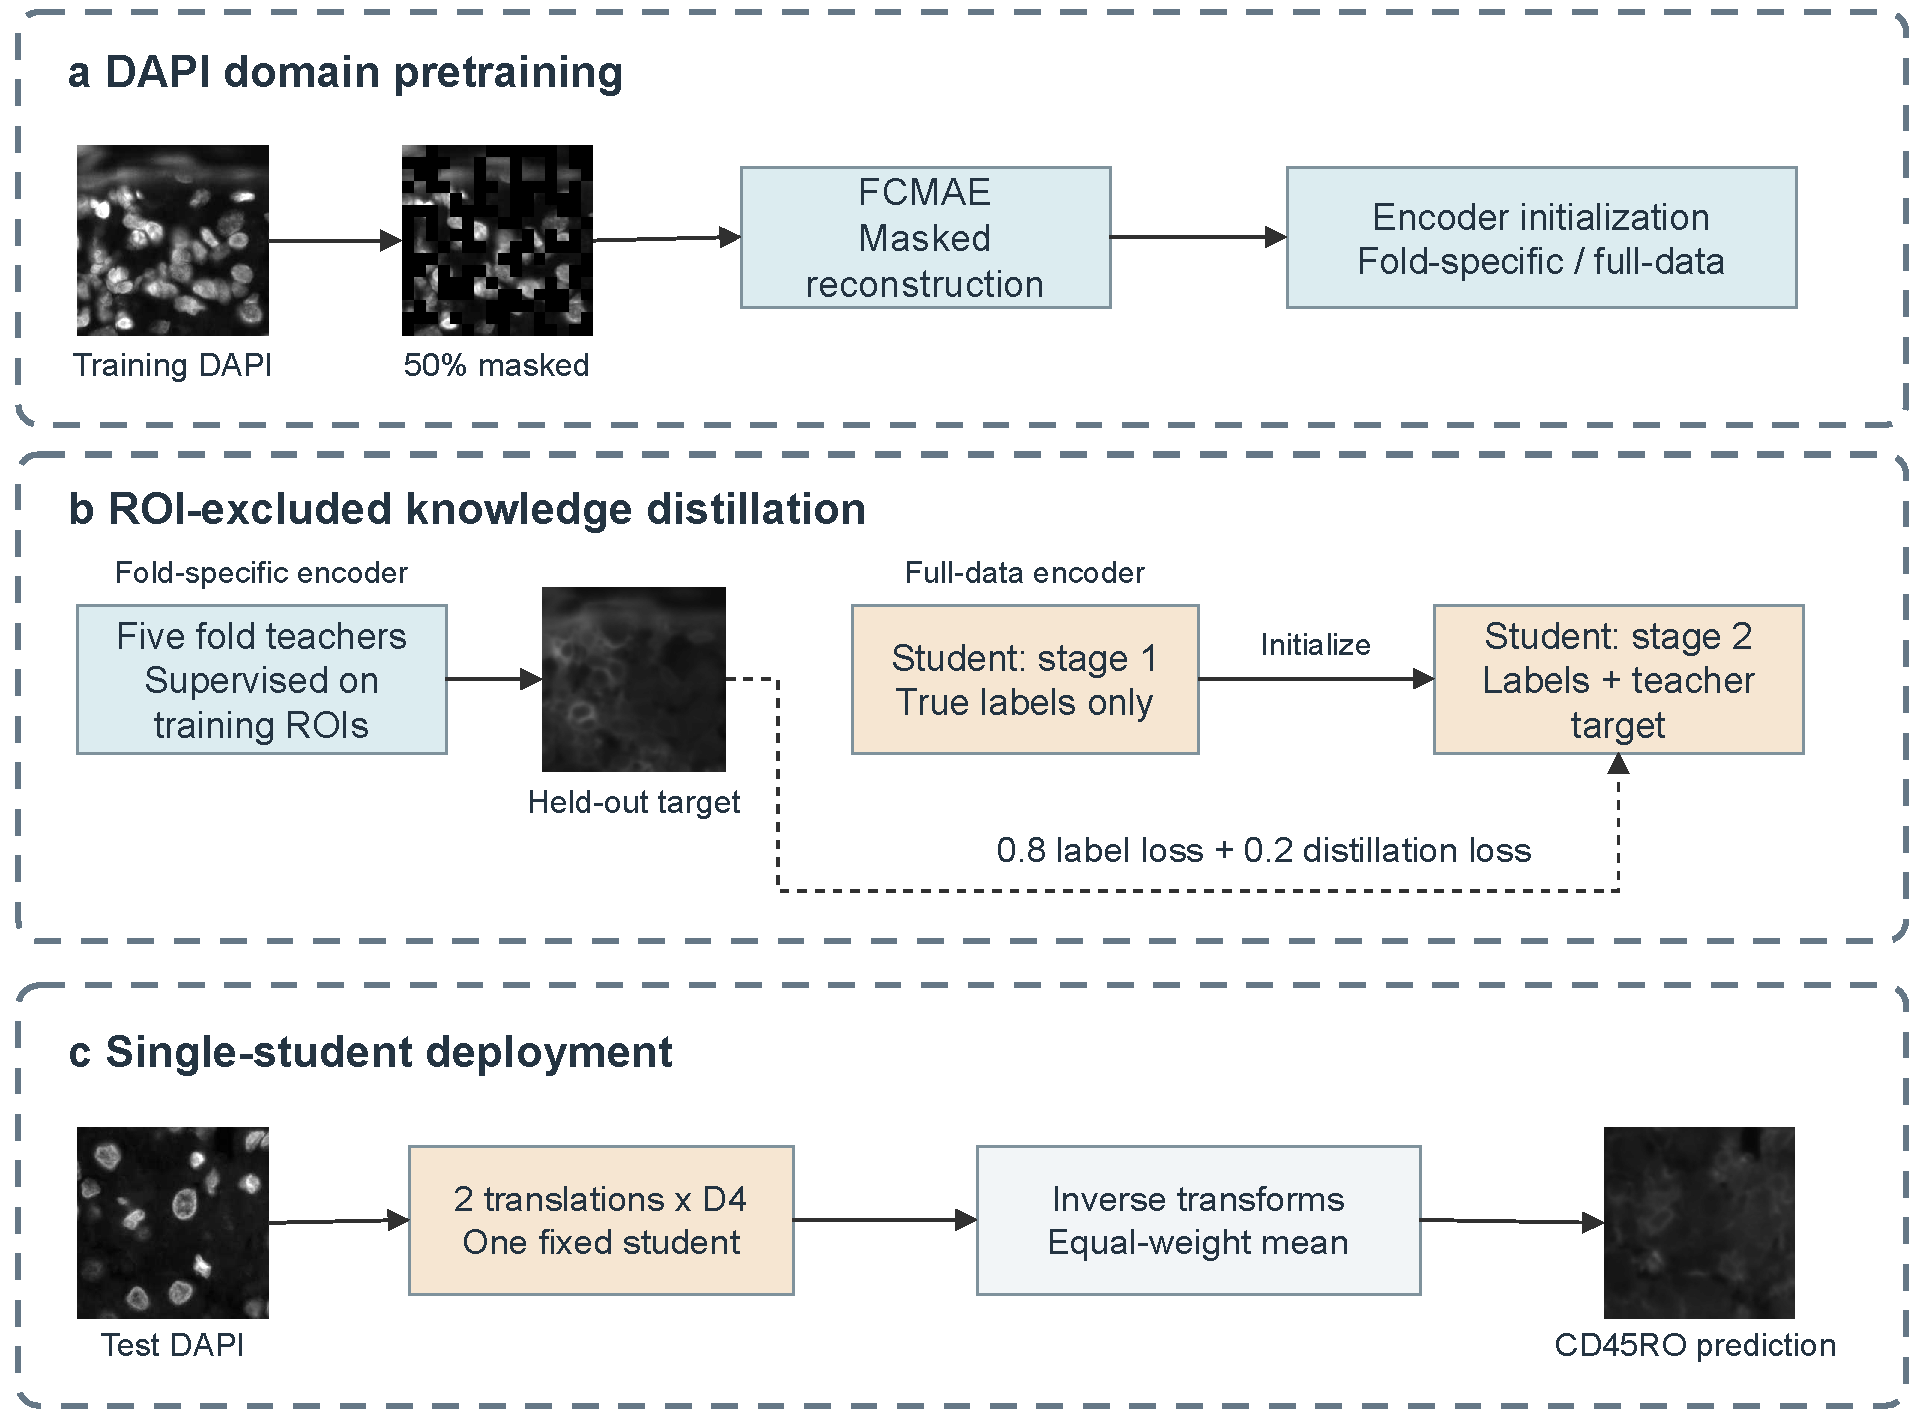
\includegraphics[width=\linewidth]{figures/workflow.pdf}
\caption{域内预训练、知识蒸馏与单模型部署流程。(a) 训练 DAPI 经随机掩码后用于重建预训练，编码器分别在各折训练 ROI 或全量训练 ROI 上学习；掩码仅为示意。(b) 每张训练图块由排除其 ROI 的教师生成 CD45RO 软目标，学生先接受真实标签监督，再进行联合蒸馏。(c) 最终学生对真实测试 DAPI 执行 16 视角预测，恢复坐标并平均，右侧为实际输出。训练示例为 ROI093\_02\_01，测试示例为 ROI025\_09\_02。图中图像统一使用 $[0,128]$ 灰度显示窗。}\label{fig:workflow}
\end{figure}

本文按“数据约定—单次前向结构—参数学习—部署推理—实验分析”的顺序展开。第\ref{sec:data}节说明 ROI 划分；第\ref{sec:model}节沿输入到输出介绍网络；第\ref{sec:training}节说明预训练、教师目标与学生优化；第\ref{sec:inference}节给出固定模型的多视角推理；第\ref{sec:results}节分析验证与平台结果；第\ref{sec:discussion}节总结方法特点和局限。

\section{数据与组织区域划分}\label{sec:data}
本节确定后续网络输入和训练验证所依据的数据范围。ROI 标识用于划分训练与验证区域，图块坐标用于读取相邻上下文和构造空间条件。
复赛训练集包含 17 个 ROI，共 2,380 张 DAPI 图块，每张配有四类免疫标记图像。测试输入包括 4 个 ROI、560 张 DAPI 图块。图块尺寸为 $256\times256$，文件名中保留 ROI 和二维网格坐标。

五折验证按完整 ROI 划分，具体见表\ref{tab:split}。每折的域内预训练与监督训练使用其余 ROI，预测覆盖该折留出区域，汇集为折外预测（out-of-fold，OOF）。最终学生使用全部 17 个训练 ROI。五折 OOF 用于评价教师配置，并为学生提供训练目标；全量学生的平台结果单独报告。两者对应不同训练范围与学习目标。

\begin{table}[H]\centering\small
\caption{五折 ROI 分组。}\label{tab:split}
\begin{tabularx}{\columnwidth}{cYr}\toprule
折 & 留出 ROI & 图块数\\\midrule
1 & 005、052、087 & 420\\
2 & 010、058、093 & 420\\
3 & 019、061、100 & 420\\
4 & 044、067、074、078 & 560\\
5 & 045、072、076、081 & 560\\\bottomrule
\end{tabularx}
\end{table}

\FloatBarrier
\section{从 DAPI 输入到标记图像输出}\label{sec:model}
在上述数据与坐标约定下，本节说明网络的一次前向计算。主路径依次为上下文输入、四级编码、瓶颈调制、逐级解码和中心裁剪；并行条件路径从同一 DAPI ROI 提取统计向量与缩略图，在瓶颈处与主路径汇合。先介绍主干编码及其基本运算，再说明条件的构造与注入，最后沿解码路径得到四通道输出。多视角预测的组合在第\ref{sec:inference}节讨论。
\subsection{上下文输入与张量约定}
以一张中心图块为预测对象，读取同 ROI 内相邻图块的像素，向四周各扩展一段上下文：
\begin{equation}
x=\mathcal H_h(I)/255,\qquad L=256+2h.
\label{eq:input}
\end{equation}
\sym{其中，$I$ 为该图块所在 ROI 的原始 DAPI 图像集合，$\mathcal H_h$ 为按网格坐标构造上下文的算子，$h$ 为每侧扩展像素数，$x\in[0,1]^{1\times L\times L}$ 为归一化网络输入，$L$ 为输入边长。训练取 $h=64$，推理取 $h=128$。}
相邻图块缺失的位置由中心图块反射填充。下文省略批量维，特征尺寸按“通道数 $\times$ 高 $\times$ 宽”书写；所有卷积和线性映射的参数均在训练中学习。图\ref{fig:architecture}展示完整前向结构。

\begin{figure}[!htbp]\centering
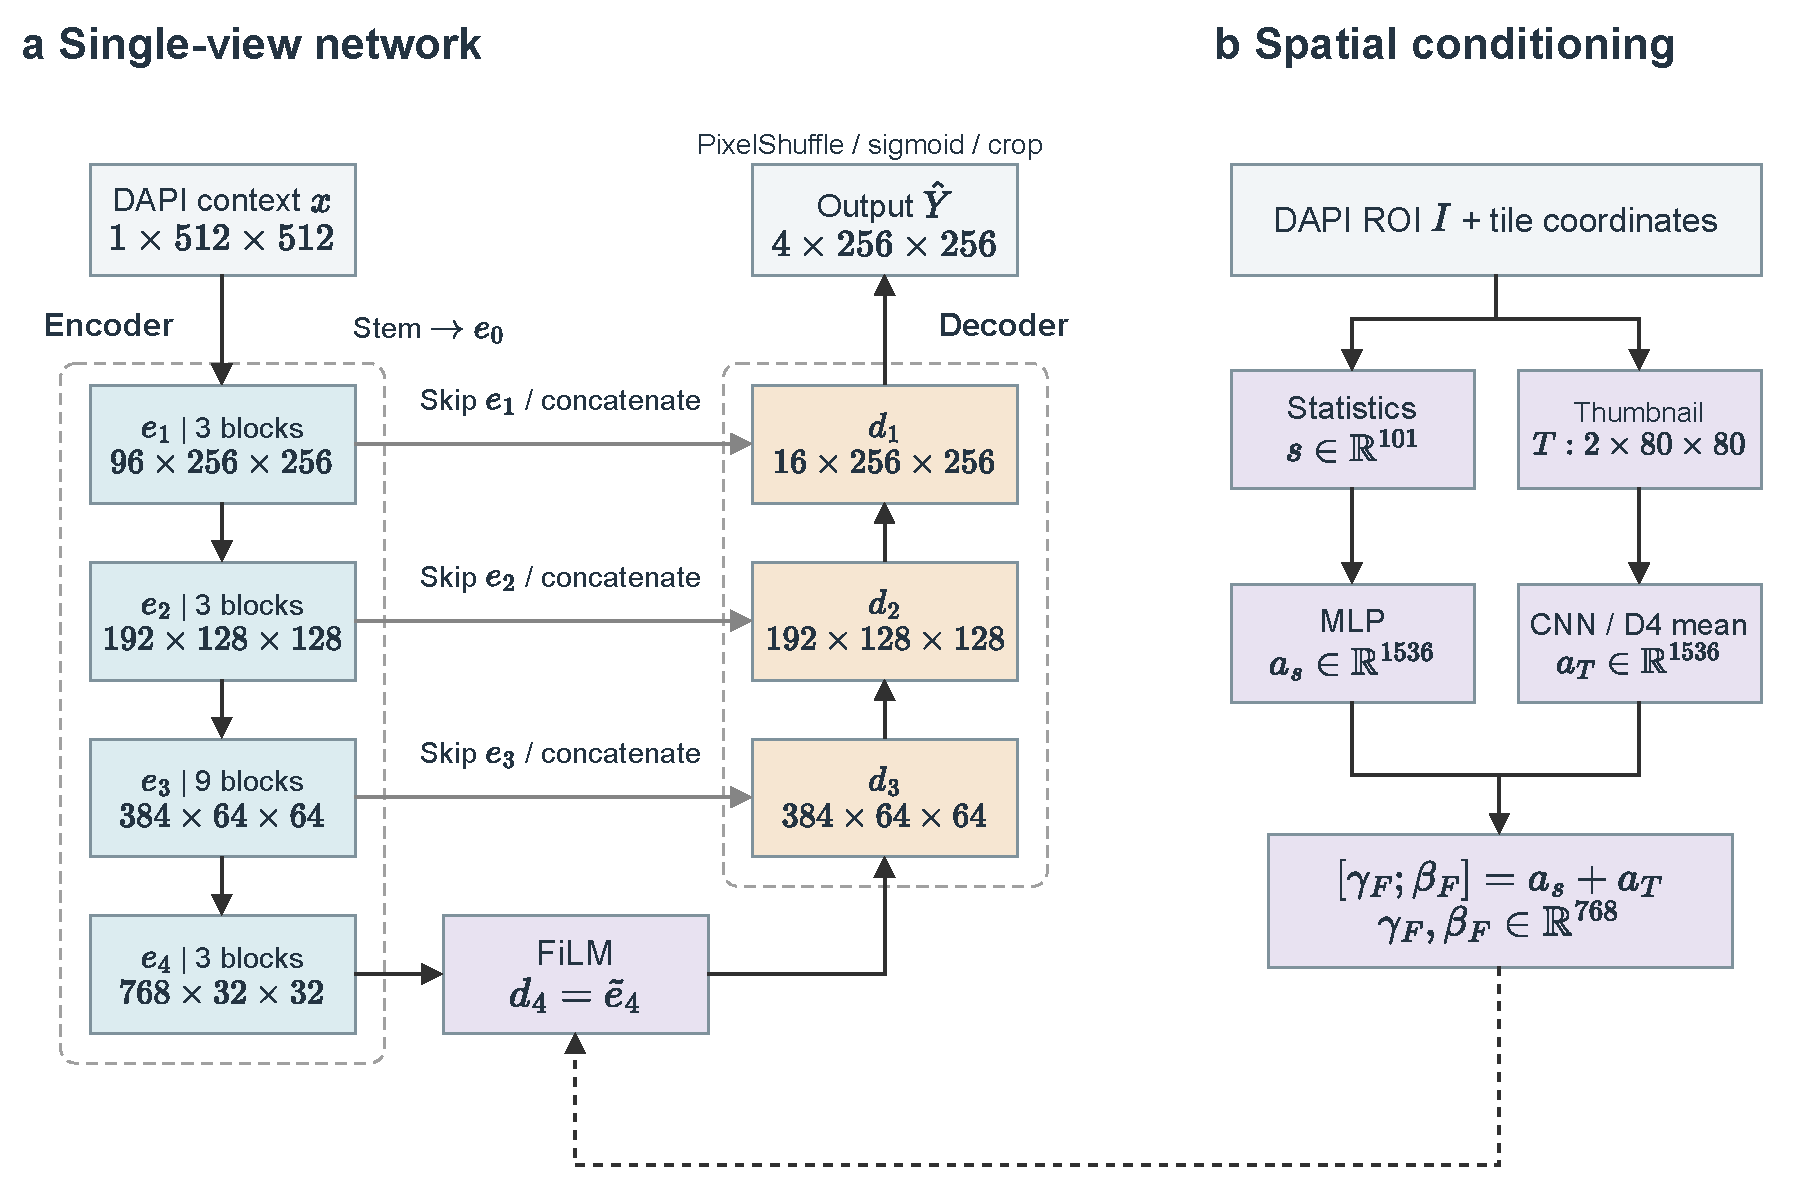
\includegraphics[width=\linewidth]{figures/architecture.pdf}
\caption{空间条件虚拟染色网络。(a) 左侧编码器逐级降低分辨率，右侧解码器通过同尺度跳跃连接恢复细节，瓶颈处注入 FiLM 条件；输出头完成像素重排、激活和中心裁剪。(b) 同一 DAPI ROI 的统计向量与邻域缩略图生成逐通道缩放和偏置，虚线将其送入瓶颈。尺寸以 $512\times512$ 推理输入为例，内部运算见图\ref{fig:block}。}\label{fig:architecture}
\end{figure}

\subsection{输入投影与四级编码器}
由上一小节得到的上下文输入 $x$ 首先进入输入投影层。该层由 $2\times2$、步长 2 的卷积和 LayerNorm 组成，将单通道图像映射为 96 通道特征。四级编码器继续构建分辨率递减的特征：
\begin{equation}
\begin{aligned}
e_0&=\op{LN}\bigl(\op{Conv}_{2,2}^{1\to96}(x)\bigr),\\
e_j&=\mathcal B_j^{[n_j]}\bigl(\mathcal A_j(e_{j-1})\bigr),
\quad j=1,2,3,4.
\end{aligned}
\label{eq:encoder}
\end{equation}
\sym{其中，$e_0$ 为输入投影特征，$e_j$ 为第 $j$ 个编码阶段的输出；$\op{Conv}_{k,s}^{a\to b}$ 表示核大小 $k$、步长 $s$、输入输出通道为 $a,b$ 的卷积；$\op{LN}$ 表示逐空间位置的通道 LayerNorm。$\mathcal A_1$ 为恒等映射，$\mathcal A_j$（$j\ge2$）依次执行 LN 和 $2\times2$ 步长 2 卷积；$\mathcal B_j^{[n_j]}$ 表示顺序堆叠 $n_j$ 个该阶段的 ConvNeXt V2 块。}
四阶段块数为 $(3,3,9,3)$，通道数为 $(96,192,384,768)$。对边长 $L$ 的输入，各阶段边长依次为 $L/2,L/4,L/8,L/16$；浅层特征同时保留给解码器跳跃连接。

\subsection{ConvNeXt V2 块内计算}
上述编码阶段中的 $\mathcal B_j$ 均由 ConvNeXt V2 块组成，解码器也复用这一基本单元。图\ref{fig:block}(a)给出块内算子顺序。每个块先做 $7\times7$ 深度卷积，再进行通道归一化与四倍扩展，最后通过 GRN 和线性投影完成残差更新：
\begin{equation}
\begin{aligned}
v&=\op{DWConv}_{7,1}(u),\\
a&=\phi\bigl(W_1\op{LN}(v)+b_1\bigr),\\
\mathcal B(u)&=u+W_2\op{GRN}(a)+b_2.
\end{aligned}
\label{eq:block}
\end{equation}
\sym{其中，$u\in\mathbb R^{C\times H\times W}$ 为块输入，$C,H,W$ 为其通道数和空间尺寸；$v$ 为逐通道深度卷积输出；$W_1,b_1$ 将每个位置的通道从 $C$ 扩展至 $4C$，$W_2,b_2$ 将其投影回 $C$。$a$ 为扩展后的激活特征；$\phi(t)=t\Phi(t)$ 为 GELU，$\Phi$ 为标准正态累积分布函数；$\op{GRN}$ 为全局响应归一化，$\mathcal B(u)$ 为块输出。}

LayerNorm\cite{layernorm}作用于每个空间位置的通道向量：
\begin{equation}
\op{LN}(v)_{c,p}=\lambda_c
\frac{v_{c,p}-\mu_p}{\sqrt{\nu_p+\epsilon_{\rm LN}}}+\delta_c.
\label{eq:ln}
\end{equation}
\sym{其中，$c$ 为通道索引，$p$ 为空间位置；$v_{c,p}$ 为该位置的特征值，$\mu_p,\nu_p$ 为该位置所有通道的均值和总体方差；$\lambda_c,\delta_c$ 为可学习仿射参数，$\epsilon_{\rm LN}=10^{-6}$ 为数值稳定常数。}

GRN 对每个扩展通道汇总空间响应，并用通道平均响应归一化\cite{convnext}：
\begin{equation}
\begin{aligned}
g_c&=\sqrt{\sum_p a_{c,p}^2},\qquad
r_c=\frac{g_c}{\frac{1}{C_a}\sum_{k=1}^{C_a}g_k+\epsilon_g},\\
\op{GRN}(a)_{c,p}&=a_{c,p}+\alpha_c a_{c,p}r_c+\beta_c.
\end{aligned}
\label{eq:grn}
\end{equation}
\sym{其中，$a_{c,p}$ 为式\eqref{eq:block}的扩展特征，$C_a=4C$ 为扩展通道数；$g_c$ 为第 $c$ 通道的空间二范数，$k$ 为求平均时的通道索引，$r_c$ 为归一化响应；$\alpha_c,\beta_c$ 为零初始化的可学习参数，$\epsilon_g=10^{-6}$。}
深度卷积保留空间局部运算，通道扩展与投影完成特征混合，残差路径维持输入信息。编码器和解码器共使用 24 个此类块。

\begin{figure}[!htbp]\centering
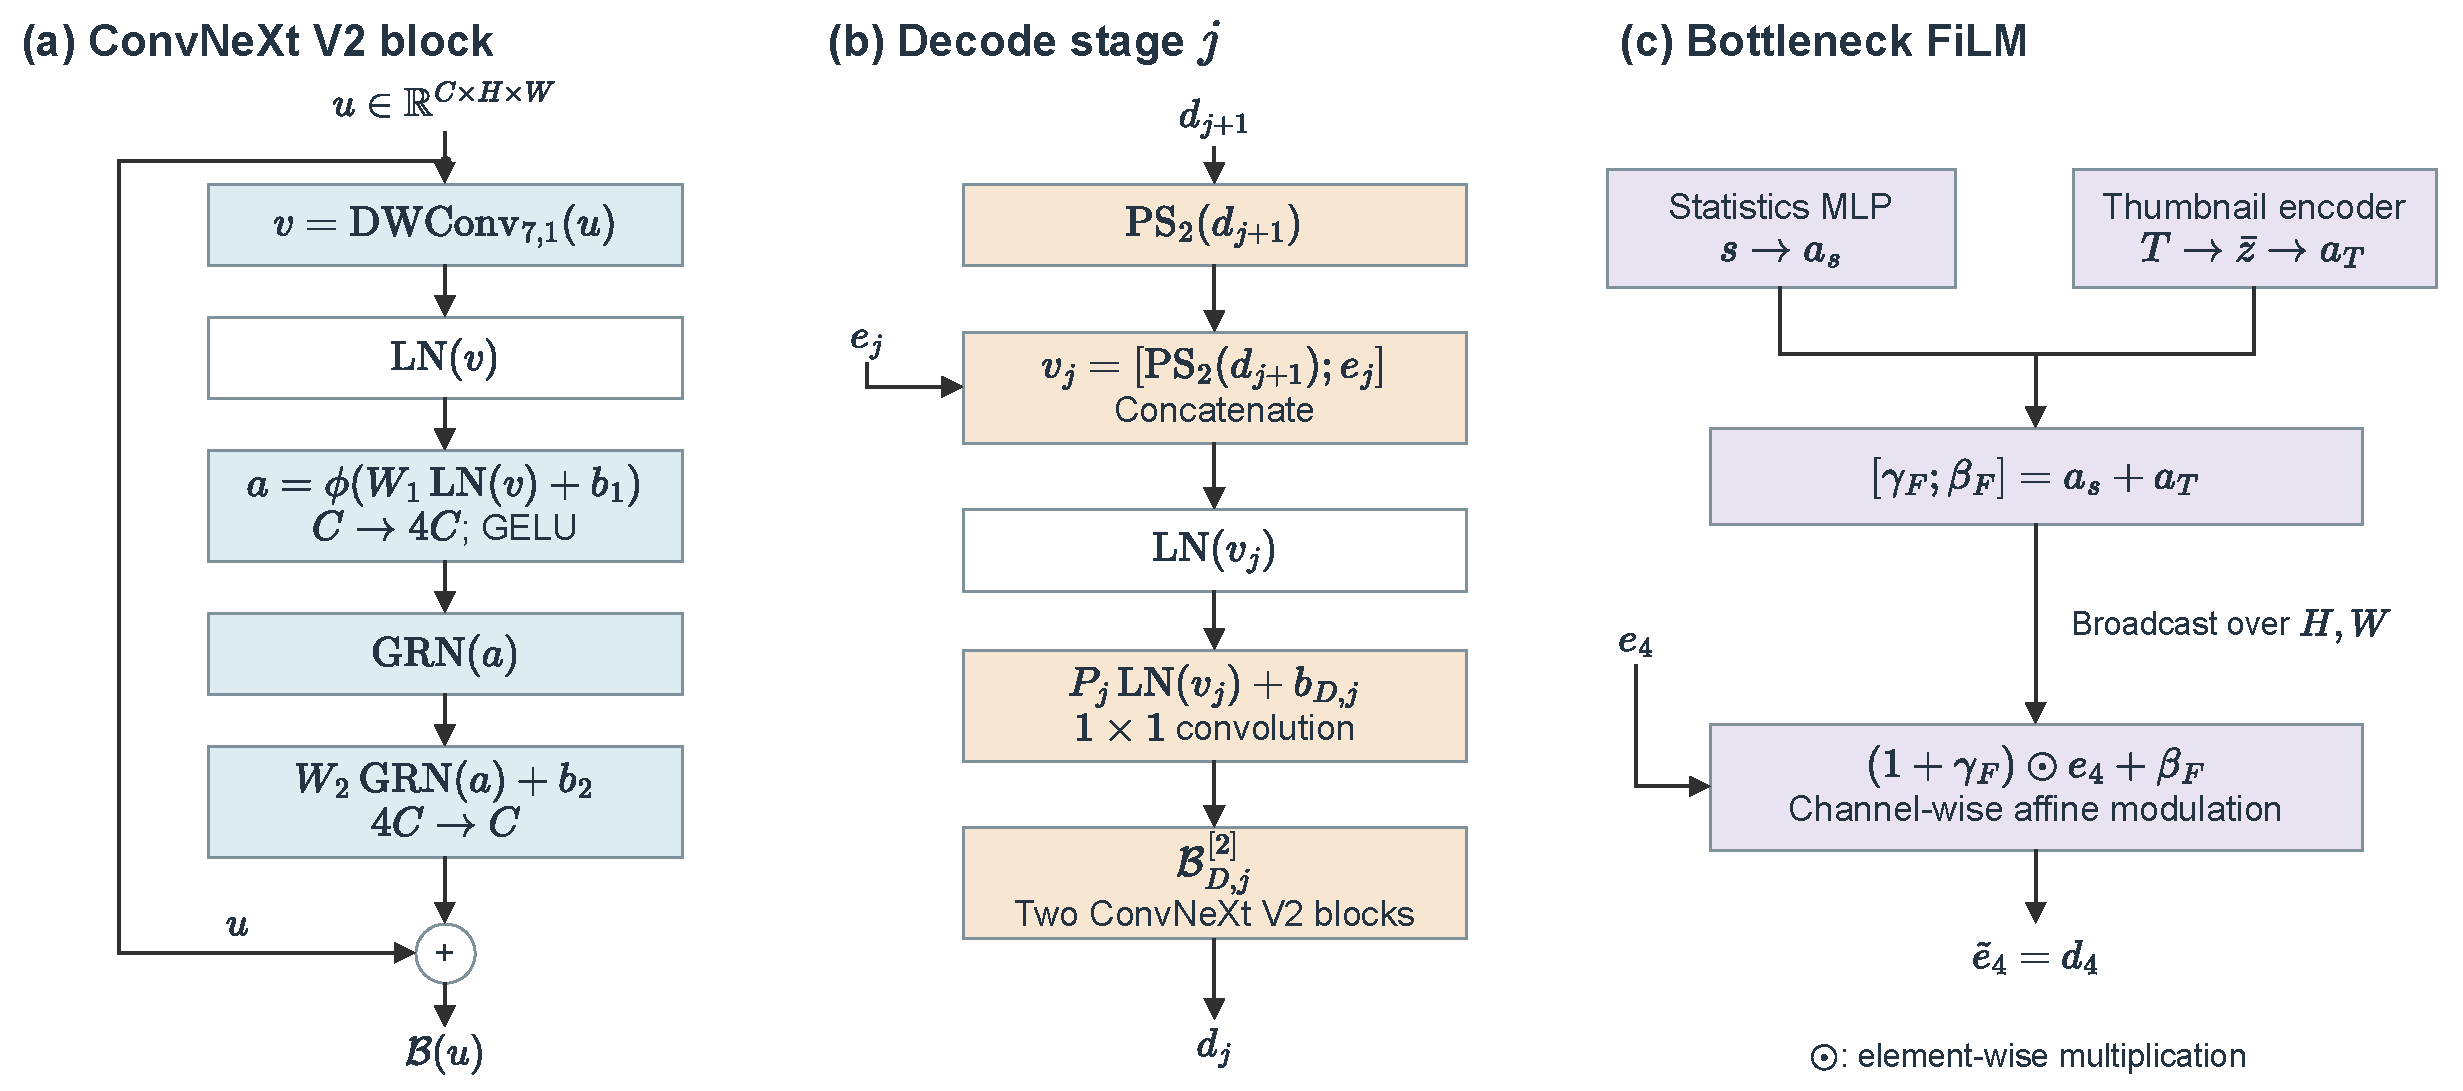
\includegraphics[width=\linewidth]{figures/blocks.pdf}
\caption{模块内部计算。(a) ConvNeXt V2 块通过深度卷积、通道扩展、GRN 与投影完成残差更新；(b) 第 $j$ 级解码依次执行像素重排、跳跃拼接、归一化、投影和两个残差块；(c) 统计与缩略图分支共同生成 FiLM 参数。}\label{fig:block}
\end{figure}

\subsection{DAPI 空间条件构造}
主干编码得到最深层特征 $e_4$ 后，网络通过条件分支引入更大范围的组织信息。该分支与主干共享 DAPI 数据来源，从中心图块及其完整 ROI 构造两类输入：101 维统计向量和双通道邻域缩略图。整体条件表示为
\begin{equation}
c=[s;\op{vec}(T)],\quad s\in\mathbb R^{101},\quad
T\in\mathbb R^{2\times80\times80}.
\label{eq:condition}
\end{equation}
\sym{其中，$c\in\mathbb R^{12901}$ 为完整条件向量，$s$ 为统计特征，$T$ 为邻域缩略图；$[\,;\,]$ 表示拼接，$\op{vec}$ 表示展开张量。条件由归一化前后的 DAPI 像素及图块坐标按固定规则计算。}

\textbf{统计分支。} 101 维特征的组成见表\ref{tab:condition}。局部强度、分位数和梯度均按 255 缩放；平均绝对梯度为横向、纵向相邻像素绝对差各自均值的平均；暗像素比例以原始灰度值不大于 5 定义。位置归一化为 $[-1,1]$，边界距离按 ROI 的网格跨度缩放，单行或单列的跨度分母取 1。邻域均值、标准差由可用图块统计，存在比例记录实际图块覆盖程度，缺失网格的强度统计与存在标志取 0。

\begin{table}[H]\centering\small
\caption{DAPI 统计条件的维度组成。}\label{tab:condition}
\begin{tabularx}{\columnwidth}{lrY}\toprule
范围 & 维度 & 内容\\\midrule
中心图块 & 9 & 均值、标准差、5 个分位数（5/25/50/75/95\%）、平均绝对梯度、暗像素比例\\
全 ROI & 11 & 行列位置、四向边界距离、网格占用率、图块均值和标准差各自的均值与标准差\\
邻域汇总 & 6 & 半径 1、2 内图块均值的均值、标准差及存在比例\\
邻域网格 & 75 & $5\times5$ 各位置的均值、标准差和存在标志\\\midrule
总计 & 101 & \\\bottomrule
\end{tabularx}
\end{table}

\textbf{缩略图分支。} 对每个邻域图块做非重叠块均值池化：
\begin{equation}
\tau_{a,b}=\frac{1}{256}\sum_{i=0}^{15}\sum_{j=0}^{15}
q_{16a+i,16b+j}.
\label{eq:thumbnail}
\end{equation}
\sym{其中，$q\in[0,1]^{256\times256}$ 为一个归一化 DAPI 图块，$\tau\in[0,1]^{16\times16}$ 为其缩略图；$a,b\in\{0,\ldots,15\}$ 为缩略图坐标，$i,j$ 为对应 $16\times16$ 原图窗口内的偏移。}
以中心图块为中心取 $5\times5$ 邻域，将 25 个缩略图按相对坐标拼成 $80\times80$ 图像，作为 $T$ 的第一个通道。第二个通道记录对应图块存在时为 1、缺失时为 0 的空间掩码。该分支覆盖最多 $1280\times1280$ 的 DAPI 范围。

\subsection{条件编码与瓶颈调制}
上一小节得到的统计向量 $s$ 和缩略图 $T$ 分别经过可学习映射，随后共同生成调制 $e_4$ 的参数。首先，统计向量经两层感知机映射为 1,536 维仿射参数：
\begin{equation}
a_s=W_{s2}\psi(W_{s1}s+b_{s1})+b_{s2}.
\label{eq:stats}
\end{equation}
\sym{其中，$a_s\in\mathbb R^{1536}$ 为统计分支输出，$s$ 为式\eqref{eq:condition}的统计向量；$W_{s1}\in\mathbb R^{256\times101}$、$W_{s2}\in\mathbb R^{1536\times256}$ 为权重，$b_{s1},b_{s2}$ 为对应偏置；$\psi(t)=t/(1+e^{-t})$ 为 SiLU 激活。}

缩略图编码器使用四层卷积，每层依次执行 $3\times3$ 步长 2 卷积、8 组 GroupNorm\cite{groupnorm}和 SiLU：
\begin{equation}
z_0=T,\qquad z_j=\psi\bigl(\op{GN}_8(K_j*z_{j-1})\bigr),
\quad j=1,\ldots,4.
\label{eq:thumbcnn}
\end{equation}
\sym{其中，$z_j$ 为第 $j$ 层缩略图特征，$K_j$ 为该层卷积核，$*$ 为卷积运算，$\op{GN}_8$ 表示每张图像独立进行的 8 组归一化，$\psi$ 为 SiLU。卷积使用一像素填充，卷积层使用无偏置卷积；四层输出通道依次为 16、32、64、64，空间边长依次为 40、20、10、5。}
GN 在每个通道组的通道和空间维计算均值与总体方差，稳定常数为 $10^{-5}$，并使用逐通道可学习缩放和偏置。

缩略图特征对八种 D4 变换求嵌入均值：
\begin{equation}
\bar z=\frac{1}{8}\sum_{g\in\mathcal G}\op{GAP}\bigl(E_T(gT)\bigr),
\quad a_T=W_T\bar z+b_T.
\label{eq:invariant}
\end{equation}
\sym{其中，$\mathcal G$ 为四个 $90^\circ$ 整数倍旋转及其镜像组成的八元素 D4 集合，$gT$ 表示对缩略图执行变换；$E_T$ 为式\eqref{eq:thumbcnn}的四层共享编码器，$\op{GAP}$ 为空间全局平均池化；$\bar z\in\mathbb R^{64}$ 为平均嵌入，$W_T\in\mathbb R^{1536\times64},b_T\in\mathbb R^{1536}$ 为线性映射参数，$a_T$ 为缩略图分支输出。}

两个条件分支相加并拆分为瓶颈的缩放和偏置：
\begin{equation}
\begin{aligned}
{}[\gamma_F;\beta_F]&=a_s+a_T,\\
\widetilde e_{4,c,p}&=(1+\gamma_{F,c})e_{4,c,p}+\beta_{F,c}.
\end{aligned}
\label{eq:film}
\end{equation}
\sym{其中，$\gamma_F,\beta_F\in\mathbb R^{768}$ 为 FiLM 参数，$a_s,a_T$ 分别由式\eqref{eq:stats}和式\eqref{eq:invariant}得到；$e_4$ 为编码器第四阶段特征，$c,p$ 为其通道和空间位置，$\widetilde e_4$ 为调制后的瓶颈。FiLM 参数在空间位置间共享。}
两分支的最终线性层权重与偏置均初始化为零，使调制层初始为恒等映射。缩略图嵌入的八视角均值用于该分支的方向不变性；101 维统计向量保留当前 ROI 坐标约定下的信息。

\subsection{跳跃连接与像素重排解码}
条件信息注入后，$\widetilde e_4$ 成为解码器的起点。解码器逐级恢复空间分辨率，并与编码阶段保留的 $e_3,e_2,e_1$ 融合：
\begin{equation}
\begin{aligned}
d_4&=\widetilde e_4,\quad
v_j=[\op{PS}_2(d_{j+1});e_j],\\
d_j&=\mathcal B_{D,j}^{[2]}\bigl(P_j\op{LN}(v_j)+b_{D,j}\bigr),
\quad j=3,2,1.
\end{aligned}
\label{eq:decoder}
\end{equation}
\sym{其中，$d_j$ 为第 $j$ 尺度的解码特征，$\op{PS}_2$ 为二倍 PixelShuffle，$e_j$ 为同尺度编码特征，$v_j$ 为通道拼接结果；$P_j,b_{D,j}$ 为 $1\times1$ 卷积权重及偏置，$\mathcal B_{D,j}^{[2]}$ 为两个串联的 ConvNeXt V2 块。}
三级拼接通道依次为 $192+384=576$、$96+192=288$ 和 $48+96=144$，经投影后依次得到 384、192、16 通道。每级先上采样，再利用浅层特征补充相应空间尺度的信息。

PixelShuffle 将通道位置重排为空间位置\cite{espcn}，二倍重排的索引定义为
\begin{equation}
\op{PS}_2(A)_{c,2i+a,2j+b}=A_{4c+2a+b,i,j}.
\label{eq:ps}
\end{equation}
\sym{其中，$A\in\mathbb R^{4C\times H\times W}$ 为输入张量，输出尺寸为 $C\times2H\times2W$；$c=0,\ldots,C-1$ 为输出通道，$i,j$ 为原空间坐标，$a,b\in\{0,1\}$ 为子像素偏移。该重排算子的可学习参数量为零。}
各解码阶段最后一个块的通道投影采用 ICNR 思路\cite{icnr}初始化：每组四个连续输出通道共享同一随机权重行，偏置置零，对应后续二倍重排的四个子像素位置。其余新建主干卷积和线性层使用标准差 0.02 的截断正态初始化。

\subsection{四通道输出与中心裁剪}
三级解码结束时，$d_1$ 的空间边长为输入的一半。输出层对其 16 个通道再做一次二倍重排，经通道偏置和 Sigmoid 生成全分辨率的四通道图像：
\begin{equation}
Y^{\rm ctx}=\sigma\bigl(\op{PS}_2(d_1)+b_o\bigr),\qquad
\hat Y=\mathcal C_{256}(Y^{\rm ctx}).
\label{eq:output}
\end{equation}
\sym{其中，$d_1\in\mathbb R^{16\times(L/2)\times(L/2)}$ 为最终解码特征，$b_o\in\mathbb R^4$ 为初始值均为 $-2$ 的可学习输出偏置；$\sigma(t)=1/(1+e^{-t})$ 为 Sigmoid，$Y^{\rm ctx}\in[0,1]^{4\times L\times L}$ 为上下文输出，$\mathcal C_{256}$ 为中心 $256\times256$ 裁剪，$\hat Y$ 为图块预测。}
四通道按 CD68、CD45RO、HLA-DR、Vimentin 排列，提交使用第二通道。末级 16 通道由四个输出通道各自对应四个子像素位置确定。监督训练时真实标签覆盖完整 $384\times384$ 上下文，教师目标约束中心 $256\times256$；推理时从 $512\times512$ 输出裁取中心图块。

\subsection{模块规模与参数分布}
上述前向路径确定了网络的全部可学习模块，表\ref{tab:params}据此汇总学生网络的逐模块参数量。编码器共 27,860,736 个参数，占约 87.74\%；解码器为 3,311,568，占约 10.43\%；空间条件模块为 581,248，占约 1.83\%；另有 4 个输出偏置。总参数量为 31,753,556。各行按互斥模块计数，包含卷积、线性层、归一化和 GRN 的可学习参数。
对式\eqref{eq:block}中的单个残差块，参数量可写为
\begin{equation}
N_{\mathcal B}(C)=8C^2+65C.
\label{eq:paramcount}
\end{equation}
\sym{其中，$N_{\mathcal B}(C)$ 为通道数 $C$ 的一个 ConvNeXt V2 块的参数总数。二次项来自两次通道线性映射，一次项包含深度卷积、线性偏置、LayerNorm 和 GRN 参数。阶段入口下采样及解码融合投影在表中另计入对应阶段。}

\begin{table}[H]\centering\small
\caption{最终学生网络的模块参数量和输出尺寸。尺寸对应单张 $512\times512$ 输入，编码阶段含其入口下采样，解码阶段含融合投影及两个残差块。}\label{tab:params}
\begin{tabularx}{\textwidth}{lYrr}\toprule
模块 & 主要配置 & 输出尺寸或维度 & 参数量\\\midrule
输入投影 & $2\times2$ 卷积，步长 2；LN & $96\times256\times256$ & 672\\
编码阶段 1 & 3 个 ConvNeXt V2 块 & $96\times256\times256$ & 239,904\\
编码阶段 2 & 下采样；3 个 ConvNeXt V2 块 & $192\times128\times128$ & 996,288\\
编码阶段 3 & 下采样；9 个 ConvNeXt V2 块 & $384\times64\times64$ & 11,137,152\\
编码阶段 4 & 下采样；3 个 ConvNeXt V2 块 & $768\times32\times32$ & 15,486,720\\\midrule
统计输入映射 & 线性层 $101\to256$；SiLU & 256 & 26,112\\
统计仿射映射 & 线性层 $256\to1536$ & 1,536 & 394,752\\
缩略图编码器 & 四层卷积 $2\to16\to32\to64\to64$；GN；SiLU & $64\times5\times5$ & 60,544\\
缩略图仿射映射 & 池化、D4 嵌入均值；线性层 $64\to1536$ & 1,536 & 99,840\\\midrule
解码阶段 3 & PixelShuffle；拼接；投影 $576\to384$；2 个块 & $384\times64\times64$ & 2,631,936\\
解码阶段 2 & PixelShuffle；拼接；投影 $288\to192$；2 个块 & $192\times128\times128$ & 670,848\\
解码阶段 1 & PixelShuffle；拼接；投影 $144\to16$；2 个块 & $16\times256\times256$ & 8,784\\
输出偏置 & 四通道可学习偏置 & 4 & 4\\
输出重排与激活 & PixelShuffle；Sigmoid & $4\times512\times512$ & 0\\\midrule
\textbf{总计} & \multicolumn{2}{l}{含编码器、条件分支、解码器与输出偏置} & \textbf{31,753,556}\\\bottomrule
\end{tabularx}
\end{table}

\FloatBarrier
\section{域内预训练与知识蒸馏}\label{sec:training}
第\ref{sec:model}节定义了网络如何生成标记图像，本节说明这些映射参数如何学习。训练包含域内预训练、教师监督学习与折外目标生成、全量学生学习三个环节。教师与学生分别从各自训练范围内的 DAPI 预训练编码器初始化；教师的两个监督阶段均使用真实标签，学生则先学习真实标签，再加入教师目标。下文依次给出预训练目标、监督损失、教师到学生的目标传递，以及各环节的优化设置。
\subsection{公开初始化及域内预训练}
训练从 ConvNeXt V2 Tiny 的 ImageNet-1K FCMAE 公开权重开始\cite{convnext}，原文件为 \nolinkurl{convnextv2_tiny_1k_224_fcmae.pt}。本模型的单通道 $2\times2$ 输入卷积按固定种子初始化，其余形状兼容的编码器参数从公开权重加载。随后在复赛训练 DAPI 上进行 800 轮域内预训练。每折使用其训练 ROI，最终学生的编码器使用全量训练 ROI。

掩码在编码器最深尺度的 $16\times16$ 网格上生成（每个网格位置对应输入的 $16\times16$ 像素区域），每张输入随机遮蔽 50\% 的网格位置，并按整数倍扩展至各特征尺度。实现采用密集张量与可见位置掩码：输入层、下采样层和块内卷积前后按可见掩码限制特征传播。预训练解码器沿用三级像素重排结构，每级使用一个块，输出一个 DAPI 重建通道。掩码区域损失为
\begin{equation}
\mathcal L_{\rm pre}=\frac{\sum_p M_p(\widetilde x_p-x_p)^2}
{\sum_p M_p}.
\label{eq:pretrain}
\end{equation}
\sym{其中，$x$ 为预训练使用的归一化 $256\times256$ DAPI 图块，$\widetilde x$ 为重建输出，$p$ 为像素位置；$M_p\in\{0,1\}$ 表示该位置属于遮蔽区域时为 1，$\mathcal L_{\rm pre}$ 为遮蔽像素上的平均平方误差。预训练完成后将编码器参数用于监督网络初始化。}
公开权重提供初始表征，域内重建训练使编码器适应本次 DAPI 的强度和形态分布。训练 DAPI 的旋转、翻转增强与掩码采样共同产生预训练样本。

\subsection{结构与像素强度联合损失}
完成域内预训练后，网络转入 DAPI 到免疫标记图像的监督学习。教师和学生共用以下结构与像素强度损失。结构相似性指标 SSIM\cite{ssim}约束局部图像结构，其窗口形式为
\begin{equation}
\op{SSIM}(a,b)=
\frac{(2\mu_a\mu_b+C_1)(2\sigma_{ab}+C_2)}
{(\mu_a^2+\mu_b^2+C_1)(\sigma_a^2+\sigma_b^2+C_2)}.
\label{eq:ssim}
\end{equation}
\sym{其中，$a,b$ 为同位置的预测和标签窗口，$\mu_a,\mu_b$ 为窗口均值，$\sigma_a^2,\sigma_b^2$ 为窗口方差，$\sigma_{ab}$ 为协方差；对 $[0,1]$ 图像取 $C_1=0.01^2,C_2=0.03^2$。图像 SSIM 为有效窗口位置的局部值均值。训练使用 $7\times7$ 均匀窗口及 $49/48$ 的样本协方差修正。}

单通道混合损失为
\begin{equation}
\begin{aligned}
\ell(\hat y,y)={}&0.7\bigl(1-\op{SSIM}_7(\hat y,y)\bigr)\\
&+\frac{0.2}{P}\sum_p|\hat y_p-y_p|
+\frac{0.1}{P}\sum_p(\hat y_p-y_p)^2.
\end{aligned}
\label{eq:loss}
\end{equation}
\sym{其中，$\hat y,y$ 为同尺寸的单通道预测与标签，$P$ 为该通道参与像素损失的像素总数，$p$ 为像素索引；$\op{SSIM}_7$ 为前述均匀 7 窗口图像 SSIM。三项分别约束局部结构、平均绝对误差和平均平方误差。}

四个输出通道的真实标签损失为
\begin{equation}
\begin{aligned}
\mathcal L_{\rm label}&=\sum_{m=1}^{4}w_m\ell(\hat y_m,y_m),\\
w&=(0.05,0.85,0.05,0.05).
\end{aligned}
\label{eq:multimarker}
\end{equation}
\sym{其中，$m$ 为按 CD68、CD45RO、HLA-DR、Vimentin 顺序排列的通道索引，$\hat y_m,y_m$ 为对应通道预测与真实标签，$w_m$ 为通道权重，$\ell$ 为式\eqref{eq:loss}。批量训练时对样本损失取平均。}

\subsection{教师目标生成与学生学习}
使用上述损失完成五折教师训练后，即可为学生生成折外回归目标。本方案采用输出层知识蒸馏\cite{distill}，以教师预测的连续灰度图像作为软目标，在图像回归空间约束学生输出。五折教师采用同一网络结构，将统计向量中 11 项全 ROI 描述固定置零，保留局部统计、邻域统计和缩略图。教师使用统一编码器学习率，在各自留出 ROI 上以八视角 D4 和上下文扩展生成 CD45RO 预测。

每张训练图像对应一个排除其 ROI 训练的教师：
\begin{equation}
t_i=\frac{1}{255}\op{round}\!\left(255\,
\mathcal V_{-k(i)}(I_i)\right).
\label{eq:target}
\end{equation}
\sym{其中，$i$ 为训练图块索引，$I_i$ 为其所在 ROI 的 DAPI 输入集合；$k(i)$ 为该 ROI 所属折，$\mathcal V_{-k(i)}$ 表示由其余折训练的教师对该图块执行八视角预测、逆变换、均值和中心裁剪后的 CD45RO 图像，值域为 $[0,1]$；$\op{round}$ 为最近整数舍入（半整数取相邻偶数），$t_i$ 为按 8 位灰度 PNG 缓存后恢复到 $[0,1]$ 的教师目标。}
教师采用第二阶段第 12 轮参数。汇集五折后，每张训练图像具有一个对应目标，共计 2,380 张。最终学生使用全部训练 ROI，保留完整 101 维统计条件：第一阶段仅优化 $\mathcal L_{\rm label}$，第二阶段通过知识蒸馏同时利用真实标签和固定教师目标，其训练目标为
\begin{equation}
\mathcal L_{\rm stu}=0.8\mathcal L_{\rm label}
+0.2\ell(\mathcal C_{256}(Y^{\rm ctx}_2),t_i).
\label{eq:student}
\end{equation}
\sym{其中，$\mathcal L_{\rm stu}$ 为学生单样本损失，$\mathcal L_{\rm label}$ 为四通道上下文标签损失；$Y^{\rm ctx}_2$ 为学生 CD45RO 上下文预测，$\mathcal C_{256}$ 为中心裁剪，$t_i$ 为式\eqref{eq:target}的教师目标，$\ell$ 为单通道混合损失；第二项为 CD45RO 中心区域的蒸馏损失。}

\subsection{优化设置与阶段衔接}
上述各环节使用 AdamW\cite{adamw} 优化，随机种子固定为 2026，具体设置见表\ref{tab:training}。教师和学生的第一阶段均训练 14 轮，第二阶段从各自第一阶段第 14 轮参数开始，重新创建优化器和余弦学习率周期。学生第一阶段使用真实标签，第二阶段加入教师目标。最终采用学生第二阶段第 12 轮参数。

监督阶段按余弦规律衰减学习率\cite{sgdr}。学生同时采用分层学习率，即按输入层和四个编码阶段的深度设置倍率，使浅层参数以较小步长更新：
\begin{equation}
\begin{aligned}
\eta_j(e)&=\rho_j\frac{\eta_0}{2}
\left[1+\cos\!\left(\frac{\pi(e-1)}{14}\right)\right],\\
\rho_j&=0.8^{4-j},\quad j=0,\ldots,4.
\end{aligned}
\label{eq:lr}
\end{equation}
\sym{其中，$e\in\{1,\ldots,14\}$ 为当前阶段训练轮次，$\eta_0$ 为该阶段基础学习率，$j=0$ 对应输入层，$j=1,\ldots,4$ 对应四个编码阶段，$\rho_j$ 为学习率倍率。解码器与条件分支使用倍率 1，教师所有编码层也使用倍率 1。第 14 轮结束后调度器衰减至 0。}
这里的分层指编码器深度，与第一、第二监督训练阶段相互独立。学生各组倍率依次为 0.4096、0.512、0.64、0.8、1.0。监督增强对 DAPI、真实标签及教师图像同步执行水平翻转、垂直翻转和 $90^\circ$ 整数倍旋转；统计条件沿用该样本的原 ROI 坐标约定，缩略图由内部 D4 嵌入均值处理方向变化。

\begin{table}[H]\centering\small
\caption{训练参数。有效批量为微批量乘梯度累积次数。}\label{tab:training}
\begin{tabularx}{\columnwidth}{lYY}\toprule
项目 & 域内预训练 & 监督训练\\\midrule
轮次 & 800 & 两阶段各 14\\
微批量 / 累积 & 8 / 4 & 4 / 4\\
基础学习率 & $2\times10^{-4}$ & $3\times10^{-4}$；$10^{-4}$\\
权重衰减 & 0.05 & $10^{-4}$\\
调度 & 10 轮预热，余弦至 $10^{-6}$ & 每阶段余弦衰减至 0\\
输入边长 & 256 & 384\\
目标 & 遮蔽位置 MSE & 结构与强度混合损失\\
掩码比例 & 0.5 & 完整输入\\
精度 & CUDA 混合精度 & CUDA 混合精度\\\bottomrule
\end{tabularx}
\end{table}

\FloatBarrier
\section{固定几何视角推理}\label{sec:inference}
上一节得到一个全量训练的学生模型。本节说明如何固定其参数，将第\ref{sec:model}节的单次前向计算扩展为完整 ROI 的多视角预测，并恢复为原网格中的输出图块。教师仅用于训练目标生成，推理读取 DAPI 及其图块坐标。
几何自集成在图像恢复中已有应用\cite{edsr}；本方案对一个学生模型使用两个完整 ROI 视角：原始坐标和内容向右、向下各平移 8 像素。每个视角内部执行八种 D4 变换。

对某个平移视角，先提取每个图块的上下文及条件，再进行 D4 预测：
\begin{equation}
Q_s=\mathcal A\!\left(
\left\{\frac18\sum_{g\in\mathcal G}\mathcal C_{256}
\left[g^{-1}f_\theta(gx_{s,i},c_{s,i})_2\right]\right\}_i
\right).
\label{eq:tta}
\end{equation}
\sym{其中，$s\in\{(0,0),(8,8)\}$ 为 ROI 平移量，$i$ 为图块索引；$x_{s,i},c_{s,i}$ 为该视角重建的归一化上下文和条件；$f_\theta$ 为参数 $\theta$ 固定的学生网络，下标 2 表示 CD45RO 通道；$g\in\mathcal G$ 为 D4 变换，$g^{-1}$ 为其逆变换，$\mathcal C_{256}$ 为中心裁剪，$\mathcal A$ 按网格坐标拼接图块，$Q_s$ 为该视角的 ROI 预测。}
同一平移视角内的统计条件保持一致，缩略图分支内部计算八视角嵌入均值；平移视角之间从变换后的完整 DAPI ROI 重新计算全部条件。两个 ROI 预测恢复坐标后等权平均：
\begin{equation}
\hat R=\tfrac12\left(Q_{(0,0)}+
\mathcal R_{(8,8)}(Q_{(8,8)})\right).
\label{eq:translate}
\end{equation}
\sym{其中，$\hat R$ 为最终 CD45RO ROI 预测，$Q_{(0,0)},Q_{(8,8)}$ 为式\eqref{eq:tta}的两个视角输出，$\mathcal R_{(8,8)}$ 将平移预测向左、向上恢复 8 像素。两个视角内各含八个等权预测，总计 16 个视角。}
ROI 平移及坐标恢复采用边缘复制；上下文图块缺失时采用式\eqref{eq:input}所述反射填充。这两个边界处理步骤分别对应完整 ROI 变换与局部图块读取。

将平均结果按原网格切分，执行固定保存转换：
\begin{equation}
J_i=\op{RGB}\left(\op{uint8}\left[
\op{clip}\bigl(\op{round}(255\hat R_i),0,255\bigr)\right]\right).
\label{eq:save}
\end{equation}
\sym{其中，$\hat R_i$ 为第 $i$ 个 $256\times256$ 预测图块，$\op{round}$ 为最近整数舍入（半整数取相邻偶数），$\op{clip}$ 将数值限制在给定闭区间，$\op{uint8}$ 为 8 位无符号整数转换，$\op{RGB}$ 将灰度复制到三个颜色通道，$J_i$ 为待保存图像。JPEG 保存质量固定为 95。}

\FloatBarrier
\section{实验结果与分析}\label{sec:results}
本节分别考察训练机制与最终部署结果。首先通过按 ROI 留出的五折预测比较域内预训练、编码器学习率和固定平移推理；随后比较教师配置，并报告全量学生的平台结果，最后展示留出 ROI 上的真实输入、标记图像与教师预测。五折实验对应未加入蒸馏的教师网络，因此其分数用于评价基础配置，不作为最终蒸馏学生的独立泛化估计。
\subsection{实验环境与指标}
训练及推理使用 NVIDIA A100 40GB、Linux、Python 3.12.13 和 PyTorch 2.8.0+cu128。分组验证采用复赛肝脏数据的五折划分，覆盖 2,380 张图块，并按图像、折和 ROI 汇总结果。

分组验证的 SSIM 按式\eqref{eq:ssim}计算，采用 $11\times11$ 高斯窗口、标准差 1.5、总体协方差和有效窗口。PSNR 及综合分数为
\begin{equation}
\begin{aligned}
\op{PSNR}_i&=10\log_{10}\frac{255^2}{\max(\op{MSE}_i,10^{-10})},\\
S&=\frac1N\sum_{i=1}^{N}\left[70\op{SSIM}_i+
0.6\op{clip}(\op{PSNR}_i,0,50)\right].
\end{aligned}
\label{eq:score}
\end{equation}
\sym{其中，$i$ 为评价图像索引，$N$ 为图像总数，$\op{MSE}_i$ 为预测与标签在 $[0,255]$ 灰度尺度上的平均平方误差，$\op{PSNR}_i$ 单位为 dB，$\op{SSIM}_i$ 为该图的结构相似度，$S$ 为本地平均综合分数；$\op{clip}$ 将单图 PSNR 截断至 $[0,50]$。}
验证预测经质量为 95 的 JPEG 编码后计算指标。

\subsection{域内预训练与学习率对照}
表\ref{tab:validation}汇总复赛验证结果。公开初始化基线使用相同主干和监督方式；加入域内预训练后，综合分数从 77.52153 增至 78.55263，增益为 1.03110，全部 17 个 ROI 改善。该对照表明，在所测试的网络和监督设置下，DAPI 重建预训练能够改善染色预测。

\begin{table}[H]\centering\small
\caption{复赛五折对照。每行比较该项改动前后对应配置，分数为 CD45RO 本地综合分。}\label{tab:validation}
\begin{tabularx}{\columnwidth}{Yrrr}\toprule
改动项 & 改动前 & 改动后 & 增益\\\midrule
DAPI 域内预训练 & 77.52153 & 78.55263 & +1.03110\\
分层学习率 & 78.55263 & 78.68642 & +0.13379\\
固定平移 TTA & 78.68642 & 78.69092 & +0.00450\\\bottomrule
\end{tabularx}
\end{table}

在域内初始化基础上，编码器分层学习率相对统一倍率进一步提升 0.13379，4/5 折和 12/17 个 ROI 改善。折间最大降幅约为 0.20100，ROI 间最大降幅约为 0.36688，说明不同组织区域对更新步长具有不同响应。

固定平移 TTA 复用相同的五折模型参数，相对八视角 D4 的综合分数增加 0.00450，3/5 折和 13/17 个 ROI 改善；平均 SSIM 增加 0.00003073，截断后平均 PSNR 增加 0.003907 dB。ROI 间最大分数降幅约为 0.03388。增加视角的验证收益较小，计算开销约为原八视角推理的两倍。

\subsection{教师配置与最终学生}
在上述完整条件模型的对照基础上，进一步比较用于目标生成的教师配置。最终使用的局部条件教师 OOF 分数为 78.73366，比采用分层学习率的完整条件教师分数 78.68642 高 0.04723，4/5 折和 11/17 个 ROI 改善。这一比较涉及条件输入和学习率配置两项差异，反映两套教师方案的整体效果。最终训练将局部条件教师目标用于保留完整条件的学生。

表\ref{tab:online}汇总全量学生的线上结果。完整条件教师目标下的学生采用八视角 D4 时为 79.0903，加入固定平移后为 79.0967。保持学生结构、第一阶段初始化和推理流程，改用局部条件教师目标后为 79.1052，相差 0.0085。

\begin{table}[H]\centering\small
\caption{全量学生的线上结果。三种配置的学生均采用分层学习率，评价通道为 CD45RO。}\label{tab:online}
\begin{tabularx}{\columnwidth}{Yrrr}\toprule
教师目标与推理视角 & Score & SSIM & PSNR\\\midrule
完整条件教师；8 视角 & 79.0903 & 0.899 & 26.929\\
完整条件教师；16 视角 & 79.0967 & 0.899 & 26.933\\
局部条件教师；16 视角 & \textbf{79.1052} & 0.899 & 26.932\\\bottomrule
\end{tabularx}
\end{table}

表中 SSIM 保留三位小数，最后两个配置的 PSNR 相差 0.001 dB；这一显示精度不足以分解综合分数变化中各指标的贡献。实验结果中，域内预训练带来较大的本地增益，教师配置与几何推理带来的平台变化较小。由于两组结果分别来自分组验证和平台测试，其增益幅度应结合各自的比较范围理解。

\subsection{真实图像的定性比较}
图\ref{fig:qualitative}并列展示真实 DAPI、CD45RO 标签及相应的 ROI 留出教师预测。三个样本按全部训练图块的 CD45RO 标签平均强度排序，取最接近第 25、50、75 百分位的位置；选择依据仅为标签强度。预测图像取自最终学生使用的折外教师缓存，包含八视角 D4 与上下文推理，其教师均未使用对应 ROI 训练。

在这些示例中，预测保留了部分较大尺度的强度分布，但标签中的细小亮点、局部高亮边缘和强度变化较预测更明显。中心裁剪进一步显示，教师输出对局部细节的恢复偏平滑。这组图用于观察教师软目标的形态及误差；最终学生的实际测试输入输出另见图\ref{fig:workflow}(c)。

\begin{figure}[!htbp]\centering
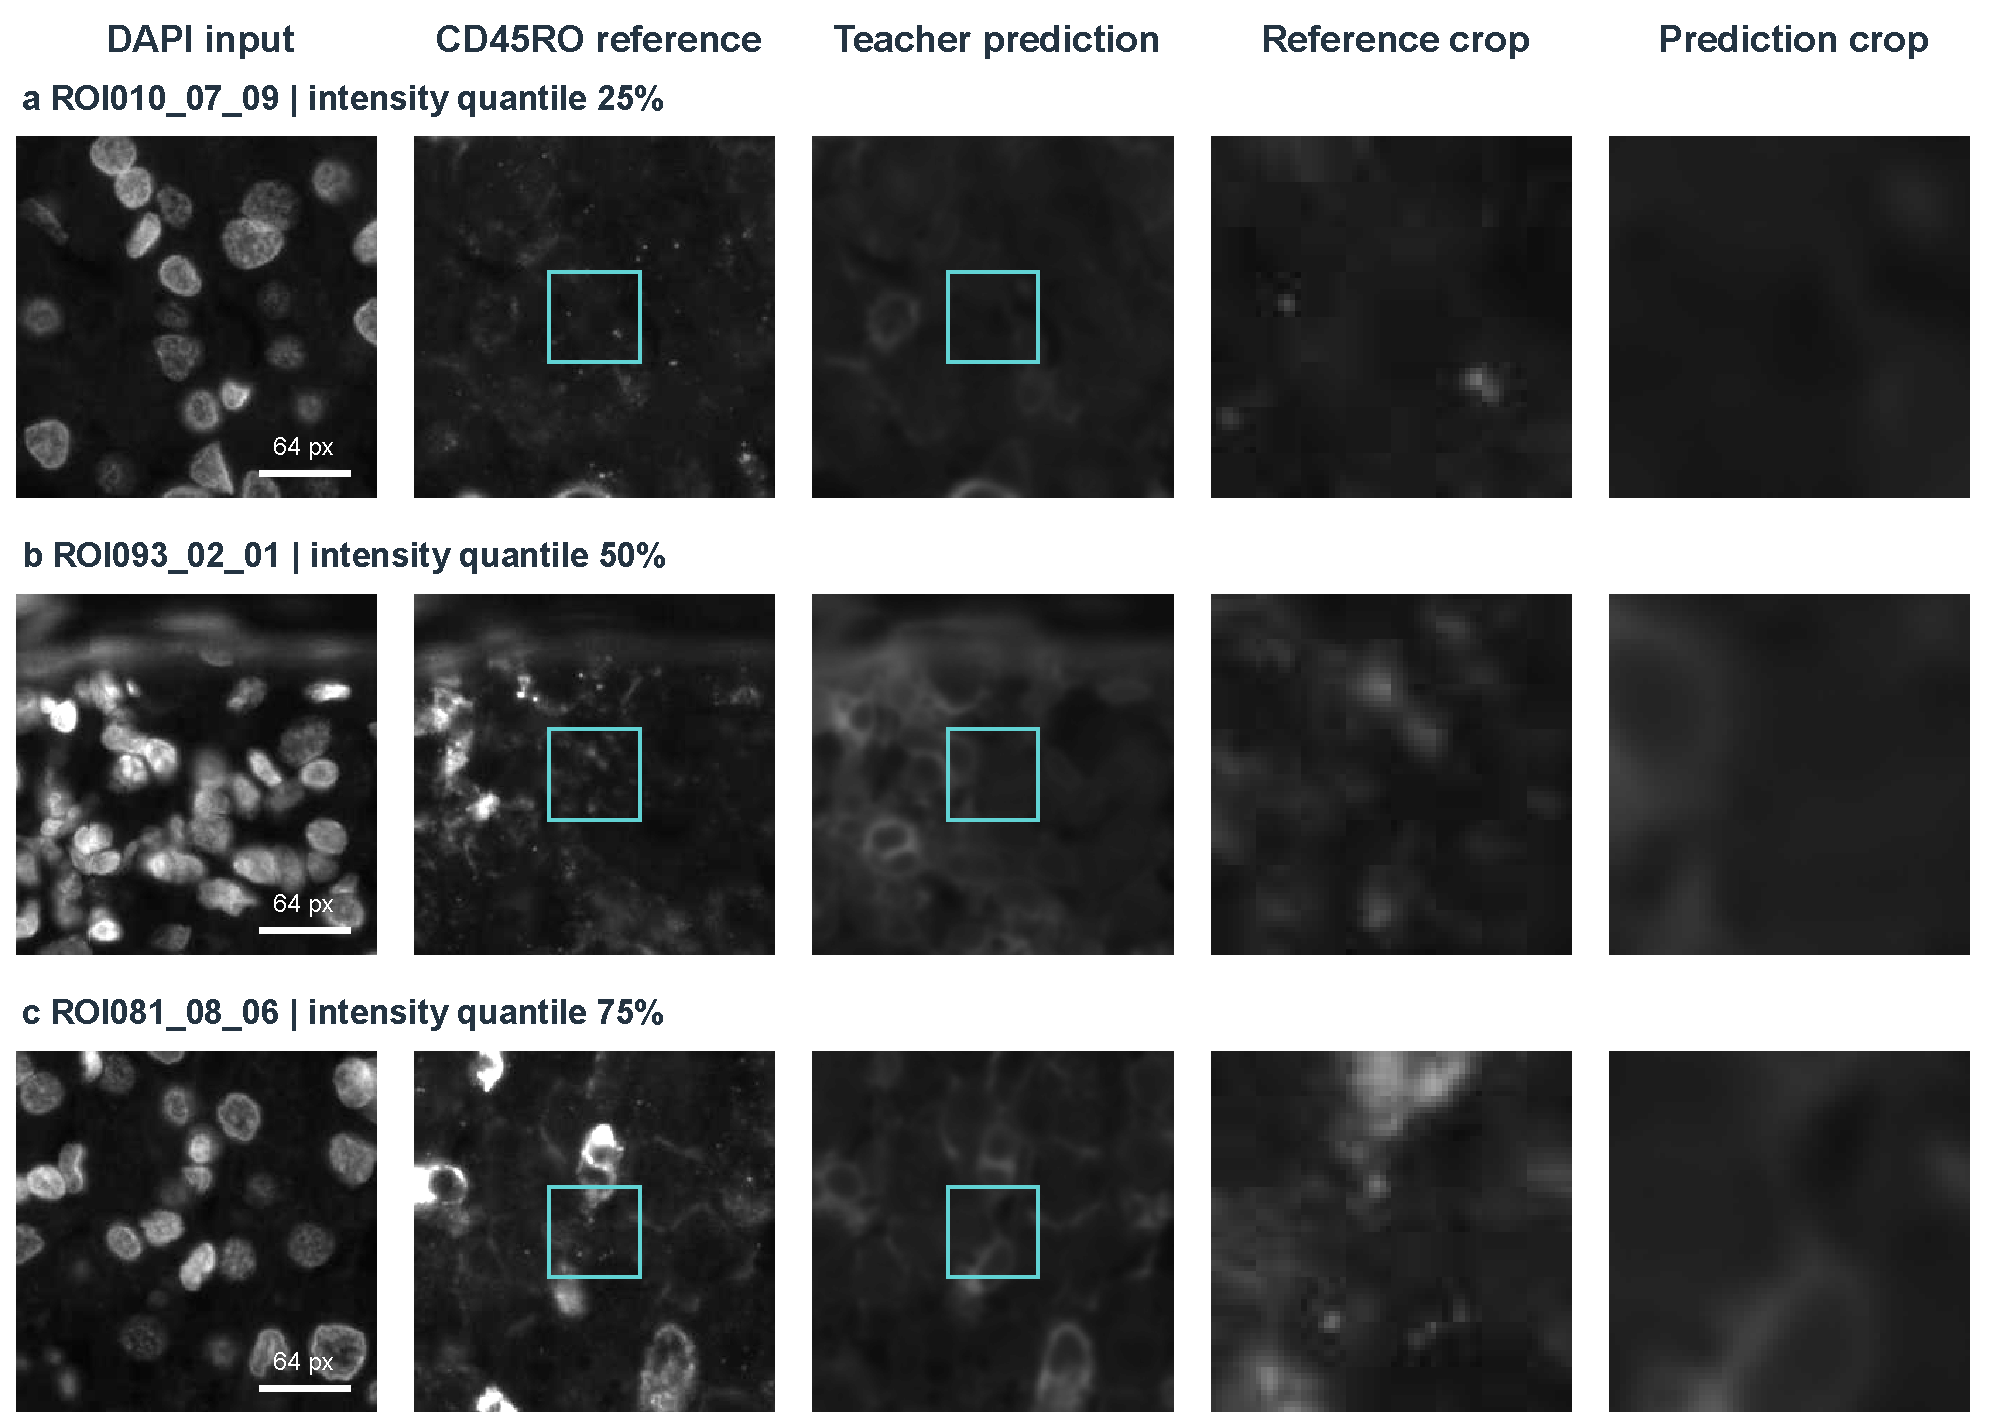
\includegraphics[width=\linewidth]{figures/qualitative.pdf}
\caption{留出 ROI 的真实配对图像与教师预测。每行从左至右依次为 DAPI 输入、真实 CD45RO、教师预测及后两者的中心 $64\times64$ 裁剪；青色方框标出相同裁剪位置，整图为 $256\times256$ 像素，比例尺为 64 像素。所有面板共用固定的 $[0,128]$ 线性灰度显示窗，仅用于可视化。教师预测为训练时采用的 8 位 PNG 软目标，未施加锐化或空间滤波。}\label{fig:qualitative}
\end{figure}

\FloatBarrier
\section{方法特点与局限}\label{sec:discussion}
结合前述结构、训练流程和实验结果，本节归纳方法的主要特点，并界定当前结果的适用范围。

\subsection{方法特点}
本方法将不同范围的 DAPI 信息汇入同一个预测网络：上下文输入与跳跃连接保留局部细节，覆盖 $5\times5$ 图块的缩略图补充较大范围的组织背景，101 维统计向量描述强度分布与空间关系。两个条件分支在瓶颈处完成调制，其参数量约占总量的 1.83\%。这种结构把局部图像恢复与组织背景建模结合在一起。

参数学习与上述结构相配合。域内掩码重建提供编码器初始化，配对标记图像建立染色映射，知识蒸馏则在第二阶段利用按 ROI 排除生成的教师目标，为学生增加回归约束。四个标记通道共享主干，CD45RO 的真实标签权重为 0.85，其余通道共同参与特征学习。完成训练后，部署使用一个约 31.75M 参数的学生网络，并通过固定几何视角平均生成最终图像。

\subsection{局限性}
当前实验基于 17 个训练 ROI，所覆盖的肝脏组织分布有限；部分改动虽提高平均分数，仍在个别折和 ROI 上出现回退。本文重点评价 CD45RO，相关结论限于该通道和本次数据。教师 OOF 与全量学生的平台结果分别提供基础配置与最终输出的证据，现有比较不足以单独量化蒸馏对学生泛化性能的贡献。

在输入和计算方面，空间条件依赖 ROI 坐标及图块邻接信息，数据缺失和外缘填充会改变可用上下文。教师目标采用 8 位量化表示，会引入量化误差；固定平移的边界复制也会影响外缘预测。16 视角推理相对八视角 D4 的计算开销约增加一倍，而本次验证中的平均增益较小，体现了精度与推理成本之间的取舍。

\begin{thebibliography}{99}\small
\setlength{\itemsep}{1pt}
\bibitem{unet} O. Ronneberger, P. Fischer, and T. Brox. U-Net: Convolutional Networks for Biomedical Image Segmentation. MICCAI, 2015. \href{https://arxiv.org/abs/1505.04597}{arXiv:1505.04597}.
\bibitem{cytoland} Z. Liu, E. Hirata-Miyasaki, S. Pradeep, et al. Robust virtual staining of landmark organelles with Cytoland. Nature Machine Intelligence, 7:901--915, 2025. \href{https://doi.org/10.1038/s42256-025-01046-2}{doi:10.1038/s42256-025-01046-2}.
\bibitem{convnext} S. Woo, S. Debnath, R. Hu, et al. ConvNeXt V2: Co-designing and Scaling ConvNets with Masked Autoencoders. CVPR, 2023. \href{https://arxiv.org/abs/2301.00808}{arXiv:2301.00808}.
\bibitem{espcn} W. Shi, J. Caballero, F. Husz\'ar, et al. Real-Time Single Image and Video Super-Resolution Using an Efficient Sub-Pixel Convolutional Neural Network. CVPR, 2016. \href{https://arxiv.org/abs/1609.05158}{arXiv:1609.05158}.
\bibitem{film} E. Perez, F. Strub, H. de Vries, V. Dumoulin, and A. Courville. FiLM: Visual Reasoning with a General Conditioning Layer. AAAI, 2018. \href{https://arxiv.org/abs/1709.07871}{arXiv:1709.07871}.
\bibitem{layernorm} J. L. Ba, J. R. Kiros, and G. E. Hinton. Layer Normalization. arXiv, 2016. \href{https://arxiv.org/abs/1607.06450}{arXiv:1607.06450}.
\bibitem{groupnorm} Y. Wu and K. He. Group Normalization. ECCV, 2018. \href{https://arxiv.org/abs/1803.08494}{arXiv:1803.08494}.
\bibitem{icnr} A. Aitken, C. Ledig, L. Theis, et al. Checkerboard artifact free sub-pixel convolution: A note on sub-pixel convolution, resize convolution and convolution resize. arXiv, 2017. \href{https://arxiv.org/abs/1707.02937}{arXiv:1707.02937}.
\bibitem{ssim} Z. Wang, A. C. Bovik, H. R. Sheikh, and E. P. Simoncelli. Image Quality Assessment: From Error Visibility to Structural Similarity. IEEE Transactions on Image Processing, 13(4):600--612, 2004. \href{https://doi.org/10.1109/TIP.2003.819861}{doi:10.1109/TIP.2003.819861}.
\bibitem{distill} G. Hinton, O. Vinyals, and J. Dean. Distilling the Knowledge in a Neural Network. arXiv, 2015. \href{https://arxiv.org/abs/1503.02531}{arXiv:1503.02531}.
\bibitem{adamw} I. Loshchilov and F. Hutter. Decoupled Weight Decay Regularization. ICLR, 2019. \href{https://arxiv.org/abs/1711.05101}{arXiv:1711.05101}.
\bibitem{sgdr} I. Loshchilov and F. Hutter. SGDR: Stochastic Gradient Descent with Warm Restarts. ICLR, 2017. \href{https://arxiv.org/abs/1608.03983}{arXiv:1608.03983}.
\bibitem{edsr} B. Lim, S. Son, H. Kim, S. Nah, and K. M. Lee. Enhanced Deep Residual Networks for Single Image Super-Resolution. CVPR Workshops, 2017. \href{https://arxiv.org/abs/1707.02921}{arXiv:1707.02921}.
\end{thebibliography}
\end{document}
